% Copyright 2004 by Till Tantau <tantau@users.sourceforge.net>.
%
% In principle, this file can be redistributed and/or modified under
% the terms of the GNU Public License, version 2.
%
% However, this file is supposed to be a template to be modified
% for your own needs. For this reason, if you use this file as a
% template and not specifically distribute it as part of a another
% package/program, I grant the extra permission to freely copy and
% modify this file as you see fit and even to delete this copyright
% notice. 

\documentclass{beamer}

% There are many different themes available for Beamer. A comprehensive
% list with examples is given here:
% http://deic.uab.es/~iblanes/beamer_gallery/index_by_theme.html
% You can uncomment the themes below if you would like to use a different
% one:
%\usetheme{AnnArbor}
%\usetheme{Antibes}
%\usetheme{Bergen}
%\usetheme{Berkeley}
%\usetheme{Berlin}
%\usetheme{Boadilla}
%\usetheme{boxes}
%\usetheme{CambridgeUS}
%\usetheme{Copenhagen}
%\usetheme{Darmstadt}
%\usetheme{default}
%\usetheme{Frankfurt}
%\usetheme{Goettingen}
%\usetheme{Hannover}
%\usetheme{Ilmenau}
%\usetheme{JuanLesPins}
%\usetheme{Luebeck}
\usetheme{Madrid}
%\usetheme{Malmoe}
%\usetheme{Marburg}
%\usetheme{Montpellier}
%\usetheme{PaloAlto}
%\usetheme{Pittsburgh}
%\usetheme{Rochester}
%\usetheme{Singapore}
%\usetheme{Szeged}
%\usetheme{Warsaw}

\usepackage{kotex}
\usepackage{braket}
\usepackage{array}
\usepackage{calc}
\usepackage{datetime}
\usepackage{dsfont}
\usepackage{amsmath}
\usepackage{listings}


\title{Lecture 4 : 행렬의 응용 }

% A subtitle is optional and this may be deleted
\subtitle{Fastcampus Math Camp}

\author{신승우}
% - Give the names in the same order as the appear in the paper.
% - Use the \inst{?} command only if the authors have different
%   affiliation.

% \institute[Universities of Somewhere and Elsewhere] % (optional, but mostly needed)
% {
  % \inst{1}%
  % Department of Computer Science\\
  % University of Somewhere
  % \and
  % \inst{2}%
  % Department of Theoretical Philosophy\\
  % University of Elsewhere}
% - Use the \inst command only if there are several affiliations.
% - Keep it simple, no one is interested in your street address.

% - Either use conference name or its abbreviation.
% - Not really informative to the audience, more for people (including
%   yourself) who are reading the slides online

\subject{Theoretical Computer Science}

% This is only inserted into the PDF information catalog. Can be left
% out. 

% If you have a file called "university-logo-filename.xxx", where xxx
% is a graphic format that can be processed by latex or pdflatex,
% resp., then you can add a logo as follows:

% \pgfdeclareimage[height=0.5cm]{university-logo}{university-logo-filename}
% \logo{\pgfuseimage{university-logo}}

% Delete this, if you do not want the table of contents to pop up at
% the beginning of each subsection:


% \AtBeginSection[]
% {
  % \begin{frame}<beamer>{Outline}
    % \tableofcontents[currentsection,hideallsubsections]
  % \end{frame}
% }

% Let's get started
\begin{document}

\begin{frame}
 \titlepage
\end{frame}

% \begin{frame}{Outline}
  % \tableofcontents[hideallsubsections]
  % % You might wish to add the option [pausesections]
% \end{frame}

% Section and subsections will appear in the presentation overview
% and table of contents.

\begin{frame}{Recap on Previous Lectures} 

\begin{itemize} 
\item 벡터/행렬의 연산 
\item 기저와 좌표계
\begin{itemize}
\item 선형독립
\item Span
\end{itemize} 
\item 역행렬 구하기 / 연립방정식 풀기 
\end{itemize}
\end{frame}

\section{행렬} 

\subsection{행렬의 Rank와 Nullity} 


% \begin{frame}{Motivation}

% 지지난 시간에, 벡터의 선형독립을 이용해서 어떤 집합에 좌표계를 부여할 수 있음을 보았다. 하지만 우리는 그 집합을 정의할 수 없었다. 즉, 아래 질문에 대답할 수 없었다. 


% \begin{itemize}
% \item 어떤 벡터 $\vec{a}$가 $span(\{\vec{v_i}|i=1,2,...,n\})$의 원소일까? 
% \item $c_i\vec{v_i} = \vec{a}$인 $c_i$가 존재할까? 
% \end{itemize}

% 여기서 두 번째 조건을 행렬을 이용하여 다음과 같이 다시 적어볼 수 있다. 

% $\left[ \begin{matrix} \vec{v_1} \vec{v_2}  ... \vec{v_n} \end{matrix} \right] \left[ \begin{matrix} c_1 \\ c_2 \\ ... \\ c_n \end{matrix} \right]  = \vec{a}$ 

% 이는 \textbf{선형방정식의 근의 존재}를 찾는 문제와 같은 문제이다! 따라서 위 문제를 풀기 위해서 row space와 column space의 개념을 도입하겠다. 

% \end{frame}

\begin{frame}{행렬의 Column Space/Row Space}
행렬의 column 벡터들의 span을 행렬의 column space, row 벡터들의 span을 row space라 한다. 행렬 A에 대해서 다음이 성립한다. 

\begin{itemize} 
\item elementary operation은 행렬의 row space를 바꾸지 않는다. 
\item A가 row echelon form이면, A의 row 벡터 중 영벡터가 아닌 벡터끼리는 서로 선형독립이다. 
\item A가 m by n 행렬이면, row space의 차원은 min(m,n) 이하이다. 
\end{itemize}

Column space에 대해서도 비슷한 정리가 성립하며, 3) row space의 차원과 column space의 차원은 언제나 같다. 
\end{frame}


% \begin{frame}{Proof for 1)}

% \end{frame}


% \begin{frame}{Proof for 2)}

% \end{frame}

\begin{frame}{행렬의 Rank/Nullity}
행렬 A에 대해서, 

\begin{itemize} 
\item 행렬의 row space의 차원을 그 행렬의 rank라고 한다. 
\item 벡터공간 $\{\vec{x}|A\vec{x} = \vec{0}\}$의 차원을 그 행렬의 nullity 라고 한다. 
\end{itemize}

이 때, 다음이 성립한다. 

\begin{itemize} 
\item rank(A) + nullity(A) = (A의 row의 갯수) 
\item rank(A) = (A의 row의 갯수)일 때, A가 invertible하다. 
\item nullity(A) = 0일 때, A가 invertible하다. 
\end{itemize}


\end{frame}




\subsection{행렬과 선형변환} 

\begin{frame}{선형변환} 

벡터공간 $V=\mathds{R}^n$에서 벡터공간 $W=\mathds{R}^m$으로의 선형변환은 V의 원소를 W의 원소로 대응시키는 함수 중 다음을 만족하는 함수를 말한다. 
\begin{itemize} 
\item $f(\vec{u} + \vec{v}) = f(\vec{u}) + f(\vec{v})$
\item $f(c\vec{u}) = c f(\vec{u}) $
\end{itemize}
\end{frame}

\begin{frame}{선형변환과 행렬} 
선형변환은 행렬로 볼 수 있다. 더 정확하게는, 1) $V=\mathds{R}^n$에서 $W=\mathds{R}^m$으로의 선형변환은 m by n 행렬로 볼 수 있다. 
\end{frame}

\begin{frame}[allowframebreaks]{Construction from Linear Transformation to Matrix  }

V의 기저 $\{\vec{v}_i\}$를 생각하자. 이 때, V의 임의의 원소인 $\vec{v}$는 다음과 같이 쓸 수 있다. 

\begin{equation} 
\vec{v} = c_i \vec{v}_i
\end{equation}

이 때, 선형변환 $f:V \rightarrow W$에 대해서 $f(\vec{v})$는 

\begin{equation}
f(\vec{v}) = f(c_i \vec{v}_i) = c_i f(\vec{v}_i)
\end{equation} 

로 생각할 수 있다. 이제, W의 기저 $\{\vec{w}_i\}$를 생각하자. $f(\vec{v}_i)$는 W의 원소이므로 다음과 같이 쓸 수 있다. 

\begin{equation}
f(\vec{v}_i) = d_ij \vec{w}_j
\end{equation} 

이에 착안해서, $d_{ij}$를 이용해서 행렬 D를 만들면, n by m 행렬이 된다. 이 행렬을 Transformation Matrix라고 한다. 이 행렬을 이용하면, $\vec{v} \in V$에 대해서 $f(\vec{v}) =  D \vec{v}$ 임을 알 수 있다. 
\end{frame}

\begin{frame}{선형변환의 예시 : 확대/축소} 
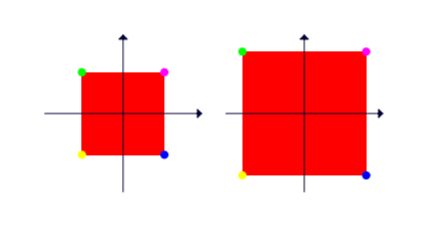
\includegraphics[width=10cm,keepaspectratio]{scale1}
\end{frame}


\begin{frame}{선형변환의 예시 : 반전}
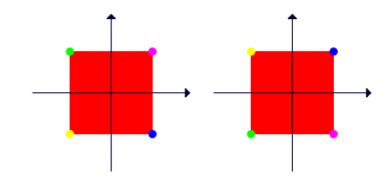
\includegraphics[width=10cm,keepaspectratio]{reflect1}
\end{frame}


\begin{frame}{선형변환의 예시 : 확대/축소}

$T_{\theta} = 
\left[ \begin{matrix}
p & 0  \\
0 & q
\end{matrix} \right] $

\begin{itemize} 
\item $p,q>1$ : 확대 
\item $0<p,q<1$ : 축소 
\item $pq<0$ : 반전 (선대칭)
\item $p<0, q<0$ : 반전 (점대칭)
\end{itemize}
\end{frame}


\begin{frame}{선형변환의 예시 : 사영} 
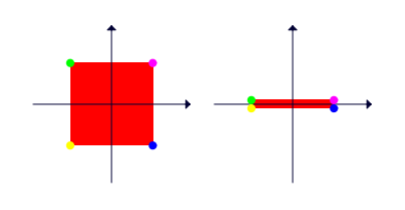
\includegraphics[width=10cm,keepaspectratio]{project1}
\end{frame}

\begin{frame}{선형변환의 예시 : 사영}

$T_{\theta} = 
\left[ \begin{matrix}
x & 0 \\
0 & y
\end{matrix} \right] $


\begin{itemize} 
\item $x=1, y=0$ : x축 사영 
\item $x=0, y=1$ : y축 사영 
\end{itemize}
\end{frame}

\begin{frame}{선형변환의 예시 : 회전변환} 
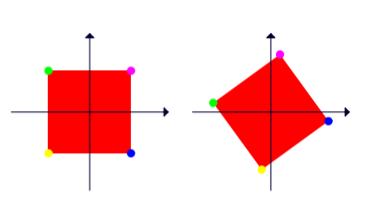
\includegraphics[width=10cm,keepaspectratio]{rotation}

\end{frame}

\begin{frame}{선형변환의 예시 : 회전변환}

$T_{\theta} = 
\left[ \begin{matrix}
cos \theta & - sin \theta  \\
sin \theta & cos \theta 
\end{matrix} \right] $


\begin{itemize} 
\item $\theta>0$ : 반시계방향으로 $\theta$만큼 회전
\item $\theta<0$ : 시계방향으로 $\theta$만큼 회전
\end{itemize}
\end{frame}



\begin{frame}{선형변환의 예시 : Orthogonal Transformation}
선형변환 $T : V \rightarrow W$ 에 대해서, V의 임의의 원소 $\vec{v}, \vec{w}$에 대해서 다음을 만족하면 Orthogonal Transformation이라고 하며, 이 때 T에 대응되는 행렬을 orthogonal matrix라고 한다. 

$\vec{v} \bullet \vec{u} = T\vec{v} \bullet T\vec{u}$ 

즉, Orthogonal Matrix는 벡터의 크기를 보존시키며 ($|\vec{v}|^2 = \vec{v} \bullet \vec{v} = T \vec{v} \bullet T \vec{v} = |T \vec{v}|^2$), 벡터 간의 각도를 보존한다. Orthogonal Transformation은 회전변환이나, 회전변환 후 반전을 하는 선형변환이다. 
\end{frame}

\begin{frame}{Orthogonal Matrix} 
n by n Orthogonal Matrix A는 다음의 특징을 가진다. 

\begin{itemize} 
\item $A^T A = A A^T = I$ \footnote{이 성질이 orthogonal matrix의 정의로 보기도 한다.}
\item $det(A) = 1$ or $det(A) = -1$ 이다. 역은 성립하지 않는다. 1인 경우, A는 회전변환이며 -1인 경우 A는 회전변환과 반전이다. 
\item A의 행벡터/열벡터는 $\mathds{R}^n$의 기저이며, 각 벡터의 크기는 모두 1이다. 
\end{itemize}
\end{frame}

\begin{frame}{행렬의 연산을 이용한 선형변환}
선형변환이라는 함수가 행렬으로 표현가능하므로, 행렬의 연산을 이용해서 선형변환을 원하는 대로 만들 수 있다. 여기서는 크게 두 가지를 살펴보고자 한다. 

\begin{itemize} 
\item 합성함수와 행렬의 곱 
\item 역함수와 역행렬
\end{itemize}

이 두 가지 예시를 회전변환을 이용해서 살펴보고자 한다. 

\end{frame}

\begin{frame}{행렬 곱과 함성함수} 

두 회전변환 

$T_{\alpha} = 
\left[ \begin{matrix}
cos \alpha & - sin \alpha  \\
sin \alpha & cos \alpha 
\end{matrix} \right] $

$T_{\beta} = 
\left[ \begin{matrix}
cos \beta & - sin \beta  \\
sin \beta & cos \beta 
\end{matrix} \right] $

가 있을 때, 두 변환행렬의 곱은 


$T_{\alpha} T_{\beta}  = 
\left[ \begin{matrix}
cos \alpha & - sin \alpha  \\
sin \alpha & cos \alpha 
\end{matrix} \right] \times 
\left[ \begin{matrix}
cos \beta & - sin \beta  \\
sin \beta & cos \beta 
\end{matrix} \right] = 
\left[ \begin{matrix}
cos \alpha cos \beta - sin \alpha sin \beta  & - cos \alpha sin \beta - sin \alpha cos \beta  \\
cos \alpha sin \beta + sin \alpha cos \beta  & cos \alpha cos \beta - sin \alpha sin \beta
\end{matrix} \right] 
 $
 
인데, 이는 삼각함수의 합차공식을 이용하면 $T_{\alpha + \beta}$임을 알 수 있다. 

\end{frame}

\begin{frame}{역행렬과 역함수} 
$T_{\alpha}$의 역행렬은 다음과 같이 구할 수 있다. 

$T_{\alpha} T^{-1}  = 
\left[ \begin{matrix}
cos \alpha & - sin \alpha  \\
sin \alpha & cos \alpha 
\end{matrix} \right] \times 
\left[ \begin{matrix}
cos \alpha & sin \alpha \\
- sin \alpha & cos \alpha
\end{matrix} \right] = I_2
$
인데, 이에서 $T^{-1} = T_{-\alpha}$임을 알 수 있다. 

\end{frame}


\subsection{행렬의 고유벡터와 고유값}

%https://math.stackexchange.com/questions/23312/what-is-the-importance-of-eigenvalues-eigenvectors

\begin{frame}{Definition of Eigen*} 
행렬 A에 대해서, 다음을 만족하는 $\lambda$와 $\vec{x}$들을 각각 고유값(eigenvalue)과 고유벡터(eigenvector)라고 한다. 
\vspace{5mm}

$ A \vec{x} = \lambda \vec{x}$ 
\vspace{5mm}
위 식을 다시 쓰면 
\vspace{5mm}
$ (A-\lambda I) \vec{x} = 0 $ 
\vspace{5mm}
이며, 여기서 $det(A-\lambda I)=0$를 특성방정식이라 한다. 이 때 특성방정식의 해는 고유값이 되며, 이에 따라 고유벡터를 계산할 수 있다. 
\vspace{5mm}
고유벡터들로 span되는 공간을 eigenspace라 한다. 
\end{frame}

\begin{frame}[allowframebreaks]{Motivation of Eigen*}
위에서 다룬 회전변환 행렬 T를 생각해 보자. 


$T_{\theta} = 
\left[ \begin{matrix}
cos \theta & - sin \theta  \\
sin \theta & cos \theta 
\end{matrix} \right] $

이 때, 회전의 축을 어떻게 구할 수 있을까? 회전의 축은 회전 전후에도 변화가 없을 것이다. 따라서, 회전의 축을 벡터 $\vec{a}$라 하면, $T\vec{a} = \vec{a}$ 임이 성립해야 한다. 이 경우, 이를 만족하는 벡터 a는 0벡터 뿐이다. 그렇다면 이는 무슨 의미를 가질까? 이는 회전축이 z축이므로, 이를 나타내는 것으로 생각할 수 있다. 

\framebreak 

이는 다음의 3차원 회전변환 행렬을 생각해보면 조금 더 명확해진다. 

$T_{\theta} = 
\left[ \begin{matrix}
cos \theta & - sin \theta & 0 \\
sin \theta & cos \theta & 0 \\ 
0&0&1
\end{matrix} \right] $

이 경우 위와 같은 방정식을 풀면 z는 어떠한 수여도 가능하고, x와 y는 0임을 알 수 있다. 즉, z축이 회전의 축임을 알 수 있다. 

이는 일반적인 선형변환에서도 같다. 어떤 선형변환 R에 대해서, $R\vec{a} = \vec{a}$가 성립한다면, 그 벡터는 선형변환에 대해서 불변이다. 즉, 어떠한 행렬의 eigenvector는 그 행렬에 대응하는 선형변환의 축이라고 볼 수 있다. 


\end{frame}

\begin{frame}{Properties of Eigen*}
일반적으로, 다음 성질들이 성립한다. 

\begin{itemize} 
\item $A^T$의 고유값과 고유벡터는 A와 같다. 
\item $A^TA$의 고유벡터는 A와 같고, 고유값은 제곱값이다. 
\item det(A)는 모든 고유값의 곱이다. 
\end{itemize}

\end{frame}

\begin{frame}[allowframebreaks]{Proof of 3)} 
어떤 행렬 A의 고유벡터를 $\vec{v}_i$, 고유값을 $\lambda_i$라 하자. 그러면 다음이 성립한다. 

\begin{eqnarray}
A \left[ \begin{matrix} 
\vec{v}_1 & \vec{v}_2 & ... & \vec{v}_n
\end{matrix} \right] 
 &=& A \left[ \begin{matrix} 
A\vec{v}_1 & A\vec{v}_2 & ... & A\vec{v}_n
\end{matrix} \right]  \\
&=& A \left[ \begin{matrix} 
\lambda_1 \vec{v}_1 & \lambda_2 \vec{v}_2 & ... & \lambda_n \vec{v}_n
\end{matrix} \right] \\
&=& \left[ \begin{matrix} 
\lambda_1 \vec{v}_1 & \lambda_2 \vec{v}_2 & ... & \lambda_n \vec{v}_n
\end{matrix} \right] 
\left[ \begin{matrix} 
\lambda_1 & 0 & ... & 0 \\
0 & \lambda_2 & ... & 0 \\
0 & 0 & ... & \lambda_n 
\end{matrix} \right] 
\end{eqnarray}

이다. 이 때, det(AB) = det(A) det(B)임을 이용하면 

\begin{eqnarray} 
& det(A) det \left( \left[ \begin{matrix} 
\vec{v}_1 & \vec{v}_2 & ... & \vec{v}_n
\end{matrix} \right]  \right) \\
= & det\left(\left[ \begin{matrix} 
\lambda_1 \vec{v}_1 & \lambda_2 \vec{v}_2 & ... & \lambda_n \vec{v}_n
\end{matrix} \right] \right)
det \left(\left[ \begin{matrix} 
\lambda_1 & 0 & ... & 0 \\
0 & \lambda_2 & ... & 0 \\
0 & 0 & ... & \lambda_n 
\end{matrix} \right] \right)\\
\end{eqnarray}

이므로, det(A)는 모든 고유값의 곱이 된다. 
\end{frame}

\begin{frame}{Eigendecomposition} 

Eigendecomposition은 어떤 행렬의 eigenvector들이 서로 선형독립일 때 가능하다. 
\begin{equation}
A \left[ \begin{matrix} 
\vec{v}_1 & \vec{v}_2 & ... & \vec{v}_n
\end{matrix} \right] 
= \left[ \begin{matrix} 
\lambda_1 \vec{v}_1 & \lambda_2 \vec{v}_2 & ... & \lambda_n \vec{v}_n
\end{matrix} \right] 
\left[ \begin{matrix} 
\lambda_1 & 0 & ... & 0 \\
0 & \lambda_2 & ... & 0 \\
0 & 0 & ... & \lambda_n \end{matrix} \right]
\end{equation}

에서, 좌변의 $\left[ \begin{matrix} 
\vec{v}_1 & \vec{v}_2 & ... & \vec{v}_n
\end{matrix} \right] $ 가 만약 역행렬을 가진다면, 다음과 같이 A를 분해할 수 있다. 

$ A = QL Q^{-1}$ 

여기서 Q는 $\left[ \begin{matrix} 
\vec{v}_1 & \vec{v}_2 & ... & \vec{v}_n
\end{matrix} \right] $ 이고, L은 $\left[ \begin{matrix} 
\lambda_1 & 0 & ... & 0 \\
0 & \lambda_2 & ... & 0 \\
0 & 0 & ... & \lambda_n \end{matrix} \right]$ 이다. 
\end{frame}

\subsection{Various Subjects on Vector/Matrix} 

\begin{frame}[allowframebreaks]{Projection} 

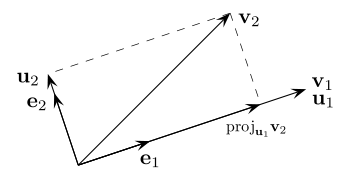
\includegraphics[width=10cm,keepaspectratio]{proj}

선형독립인 두 벡터 $\vec{v}_1, \vec{v}_2$에 대해서 $proj_{\vec{v_1}}\vec{v}_2$는 다음과 같이 정의된다. 

$\frac{\vec{v}_1 \bullet \vec{v}_2 }{\vec{v}_1 \bullet \vec{v}_1} \vec{v}_1$ 

그림에서 볼 수 있듯이, 이는 벡터 $\vec{v}_2$의 $\vec{v}_1$ 방향으로의 성분을 나타낸다. 

\framebreak
또한, $( \vec{v}_2 - proj_{\vec{v_1}}\vec{v}_2 ) \bullet \vec{v}_1 = 0$ 이다. 
\vspace{5mm}
이에서 보면 알 수 있듯이, 사영을 통해서 두 선형독립인 벡터들 $V = \{ \vec{v}_1, \vec{v}_2\}$를 서로 수직인 벡터 $W = \{ \vec{v}_1, proj_{\vec{v_1}}\vec{v}_2\}$으로 바꿀 수 있다. 또한 W의 원소들을 각각 그 원소의 크기로 나눔으로써 크기가 1이고 서로 수직한 벡터로 만들 수 있다. 
\end{frame} 

\begin{frame}[allowframebreaks]{Gram-Schmidt Process}
위 과정을 선형독립인 벡터 n개에 대해서 다음과 같이 시행하는 과정을 Gram-Schmidt Process라고 한다. 즉, 선형독립인 벡터 $\{\vec{v}_i\}$에 대해서

$\vec{u_1} = \vec{v_1},  \vec{e_1} = \frac{\vec{u_1}}{|\vec{u_1}|}$\\
$\vec{u_2} = \vec{v_2} - proj_{\vec{v_1}}\vec{v_2},  \vec{e_2} = \frac{\vec{u_2}}{|\vec{u_2}|} $ \\ 
$\vec{u_3} = \vec{v_3} - proj_{\vec{v_1}}\vec{v_3}- proj_{\vec{v_2}}\vec{v_3},  \vec{e_3} = \frac{\vec{u_3}}{|\vec{u_3}|}$ 

와 같이 $\{\vec{e}_i\}$ 를 만들 수 있다. 이 때, 기존의 벡터 $\vec{v_i}$를 새로 얻은 벡터들 $\vec{e_i}$로 다음과 같이 나타낼 수 있다. 

\begin{centering}

$\vec{v_1} = \vec{v_1} \bullet \vec{e_1} \vec{e_1}$ \\ 
$\vec{v_2} = \vec{v_1} \bullet \vec{e_1} \vec{e_1} + \vec{v_1} \bullet \vec{e_2} \vec{e_2}$ \\ 
$\vec{v_3} = \vec{v_3} \bullet \vec{e_1} \vec{e_1} + \vec{v_3} \bullet \vec{e_2} \vec{e_2} + \vec{v_3} \bullet \vec{e_3} \vec{e_3}$ 

\end{centering}

이를 행렬을 이용하여 다시 써 보면, 다음과 같이 나타낼 수 있다. 

\framebreak

$V = QR$

여기서, 
\vspace{5mm}

$V = \left[ \vec{v_1} \vec{v_2} ... \vec{v_n}  \right]$ \\ 
$Q = \left[ \vec{e_1} \vec{e_2} ... \vec{e_n} \right]$ 

$R = \left[ \begin{matrix} 
\vec{e_1}\bullet \vec{v_1} & \vec{e_1}\bullet \vec{v_2} & \vec{e_1}\bullet\vec{v_3}& ... & \vec{e_1}\bullet \vec{v_n}  \\ 
0 & \vec{e_2}\bullet\vec{v_2} & \vec{e_2}\bullet\vec{v_3} & ... & \vec{e_2}\bullet \vec{v_n} \\
0 & 0 & \vec{e_3}\bullet\vec{v_3} & ... & \vec{e_3}\bullet \vec{v_n} \\
...&...&...&...&... 
\end{matrix} \right]$

\end{frame}


\begin{frame}{QR decomposition} 
위에서와 같이 Gram-Schmidt 과정을 거쳐, Orthonormal\footnote{서로 orthogonal하며, 모두의 크기가 1인 벡터 집합}한 벡터집합을 만들 수 있으며, 이 과정에서 위 식 $V=QR$과 같이 어떤 행렬을 두 행렬의 곱으로 분해할 수 있다. 이러한 분해를 QR decomposition이라고 한다. 이 때 이러한 분해가 가능하기 위해서는 

\begin{itemize} 
\item V의 각 column 벡터들이 서로 선형 독립이여야 한다. 
\end{itemize}
\end{frame}

\begin{frame}{실습 : 위 메소드들 구현해보기} 

다음의 함수들을 짜면 됩니다. 

\begin{itemize} 
\item rank of a matrix (rank method on PyMatrix)
\item linear independence of a vector set (linearly\_independent on PyVector)
\item projection of a vector (proj method on PyVector)
\item gram-schmidt process (gram\_schmidet method on PyVector)
\item QR decomposition (QR method on PyMatrix)
\end{itemize}

\end{frame}


\begin{frame}{실습 : Rank}

구현 순서는 다음과 같다. 
\begin{itemize} 
\item PyVector에서 is\_zero() 메소드를 구현 
\item Gaussian Elimination을 통해서 reduced row echelon form을 만듬 
\item 위 결과물에서 nonzero row의 갯수를 센 후 반환
\end{itemize}
\end{frame}


\begin{frame}{실습 : Linearly Independent}

구현 순서는 다음과 같다. 
\begin{itemize} 
\item 주어진 벡터들을 row로 가지는 행렬을 생성 
\item 행렬의 rank와 row의 갯수를 비교. 같으면 True, 틀리면 False 반환. 
\end{itemize}
\end{frame}



\begin{frame}{실습 : Projection}

구현 순서는 다음과 같다. 
\begin{itemize} 
\item 정의에 따라 구현 
\end{itemize}
\end{frame}


\begin{frame}{실습 : Gram-Schmidt Process}

구현 순서는 다음과 같다. 
\begin{itemize} 
\item 들어온 벡터의 리스트가 선형독립인지 체크 
\item 정의에 따라 벡터를 생성함
\item 생성된 벡터를 크기를 1로 만들어 반환 
\end{itemize}
\end{frame}


\begin{frame}{실습 : QR decomposition}

구현 순서는 다음과 같다. 
\begin{itemize} 
\item 주어진 행렬의 column 벡터들이 선형독립인지 체크 
\item Gram-Schmidt를 이용해서 행렬의 column 벡터들을 orthonormal한 벡터들로 바꿈 
\item 위 과정에서 얻은 벡터들을 column으로 하는 행렬 Q 생성
\item R 행렬의 정의에 따라 다음과 같이 R 행렬 생성 
\begin{itemize} 
\item 행렬의 각 column을 앞부분에는 self.cols와 Q.cols의 \textit{적절한} 내적으로 채움 
\item 뒷부분은 0으로 채움 
\item 생성된 column으로 행렬 생성 
\end{itemize}
\item Q, R 반환
\end{itemize}
\end{frame}

% \begin{frame}{QR decomposition : Rectangular Case} 

% \end{frame} 

% \begin{frame}{Revisit Eigendecomposition} 

% \end{frame}

% \begin{frame}{Singular Value Decomposition} 
% m by n 행렬 M을 다음과 같은 형태로 분해하는 것을 말한다. 

% $M = U \Sigma V^T$ 

% 이 때, 

% \begin{itemize} 
% \item U : m by m Orthogonal Matrix
% \item $\Sigma$ : m by n 대각행렬
% \item $V^T$ : n by n Orthogonal Matrix \footnote{unitary matrix는 복소수 범위까지 확장될 때 해당되며, 여기서는 실수 범위만 다룰 것이므로 unitary matrix는 orthogonal matrix가 된다.}
% \end{itemize}

% \end{frame}


% \section{행렬과 벡터의 응용} 

% https://math.stackexchange.com/questions/1520832/real-life-examples-for-eigenvalues-eigenvectors


% \begin{frame}{Perspective Change Using Matrix} 

% \end{frame}

\begin{frame}{일차방정식 Solver 만들기} 

일차방정식들 $a_{ij}x_j = b_i, i,j = 1,2,...,n$을 다음과 같이 쓸 수 있다. 

$A\vec{x} = \vec{b}$

여기서 $A_{ij} = a_{ij}, \vec{x}[i] = x_i, \vec{b}[i] = b_i$이다. 이때, 일차방정식의 해 $\vec{x}$는 다음과 같은 과정을 통해서 구할 수 있다. 

\begin{itemize} 
\item A의 역행렬을 구한다. 
\begin{itemize} 
\item 만약 실패하면 해가 없거나 무한히 많은 것이다. 
\item 성공하면, $A^{-1} \vec{b}$ 를 계산한다. 
\end{itemize}
\end{itemize}
\end{frame}

\begin{frame}{일차방정식 Solver 만들기 : QR decomposition을 이용} 

$A\vec{x} = \vec{b}$

여기서 $A_{ij} = a_{ij}, \vec{x}[i] = x_i, \vec{b}[i] = b_i$이다. 이때, 일차방정식의 해 $\vec{x}$는 다음과 같은 과정을 통해서 구할 수 있다. 

\begin{itemize} 
\item A = QR로 분해한다.  
\begin{itemize} 
\item 만약 실패하면 해가 없거나 무한히 많은 것이다. 
\item 성공하면, $A\vec{x} =\vec{b}$ 양변에 $Q^T$를 곱한다. Q는 orthogonal matrix이므로 $QQ^T=I$이다. 따라서 $R\vec{x} = Q^T\vec{b}$ 이다. R은 삼각행렬이므로 어렵지 않게 $\vec{x}$를 구할 수 있다. 
\end{itemize}
\end{itemize}
\end{frame}


% \begin{frame}{Principal Component Analysis} 
% 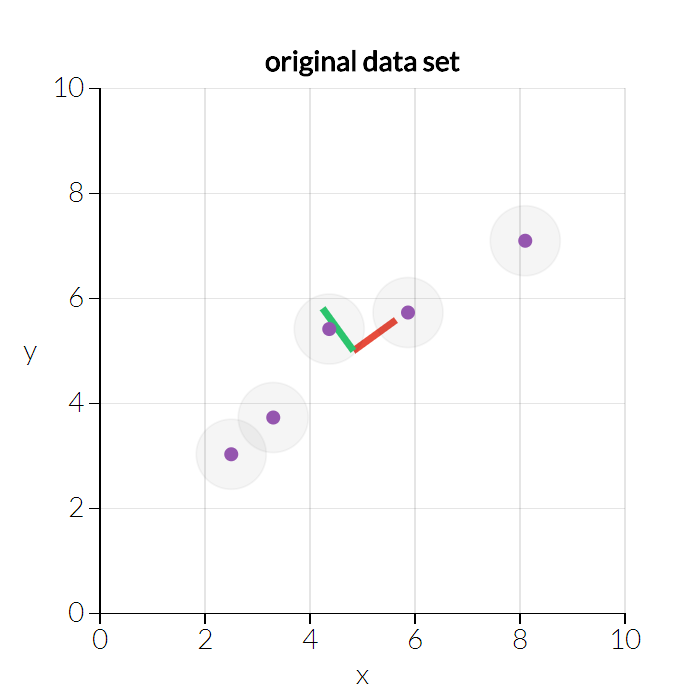
\includegraphics[height=8cm,keepaspectratio]{pcabefore}
% \end{frame}

% \begin{frame}{Principal Component Analysis} 
% 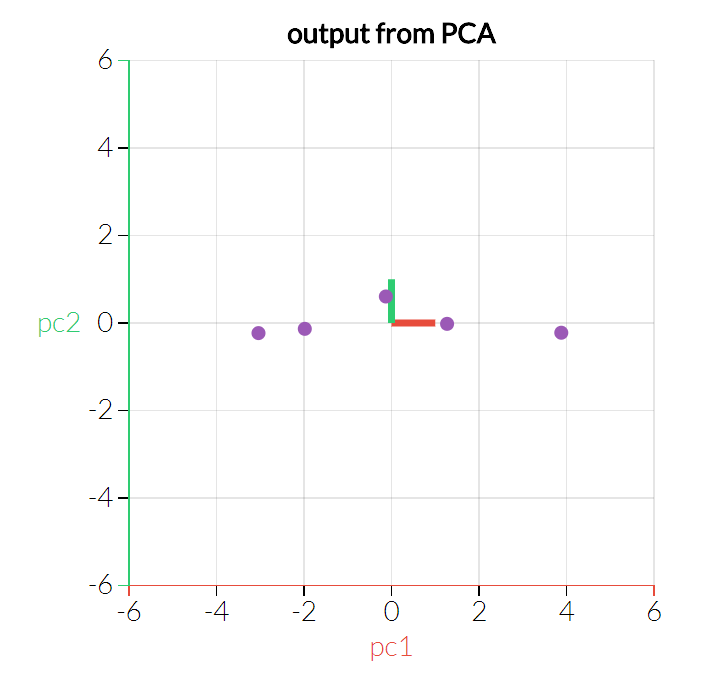
\includegraphics[height=8cm,keepaspectratio]{pcaafter}
% \end{frame}

% \begin{frame}{Principal Component Analysis} 

% \end{frame}

\begin{frame}{Linear Least Squares} 

위에서는 n by n 행렬 A와 n벡터 $\vec{x}, \vec{b}$에 대해서 $A\vec{x} = \vec{b}$인 경우에, $\vec{x}$를 찾는 방법을 알아보았다. 이번에는 m by n 행렬 A와 m벡터 $\vec{b}$에 대해서 $A\vec{x} \approx \vec{b}$ 를 만족하는 n벡터 $\vec{x}$를 찾아보자. \footnote{만약 m=n인 경우라면, 위의 선형방정식 풀이 문제가 되므로 이 문제는 선형방정식 풀이의 일반화된 문제라고 볼 수 있다.} 

여기서, $\approx$의 기준을 다음과 같이 잡자. 

\vspace{5mm}

$ min_{\vec{x}} |A\vec{x} - \vec{b}|^2 $ 

\vspace{5mm}

즉, $|A\vec{x} - \vec{b}|^2 $ 값을 최소로 하는 $\vec{x}$를 찾아보자. 
\vspace{5mm}
이러한 문제를 Linear Least Squares라 한다. 

\end{frame}


\begin{frame}{Motivation : Linear Regression} 
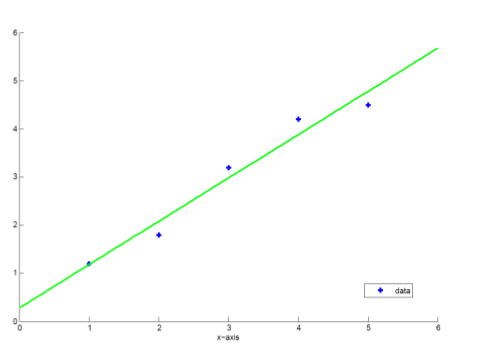
\includegraphics[height=5cm,keepaspectratio]{lin}

데이터 $(x_i, y_i), i=1,2,...,n$이 주어졌을 때, 이 데이터를 가장 잘 설명하는 $y(x) = ax + b$를 찾아보자. 
\end{frame}

\begin{frame}[allowframebreaks]{Motivation : Linear Regression} 
이 때, 문제를 다음과 같이 볼 수 있다. \\  
\vspace{5mm}

$\sum^n_{i=1} (ax_i + b - y_i)^2 $이 최소가 되는 a,b는 무엇일까? \\ 

\vspace{5mm}
이 문제를 행렬로 풀어 쓰면, 다음과 같이 생각할 수 있다. 
\framebreak
$ A = \left[ \begin{matrix} 
x_1 & 1 \\
x_2 & 1 \\ 
... & ... \\
x_n & 1 \end{matrix} \right] \in \mathds{R}^{m \times 2}, 
\vec{y} = \left[ \begin{matrix} 
y_1 \\ 
y_2 \\ 
... \\ 
y_n \end{matrix} \right] \in \mathds{R}^{m} $

라고 하면, 

$\left|A \left[ \begin{matrix} a \\ b \end{matrix} \right]  - \vec{y}\right|^2$ 를 최소화하는 문제가 된다. 즉, 저 직선을 예측하는 문제는 곧 LLS 문제를 푸는 것이 된다. 

이제, 위 문제를 조금 더 확장해 보자. 
\end{frame}


\begin{frame}{Motivation : Polynomial Regression} 
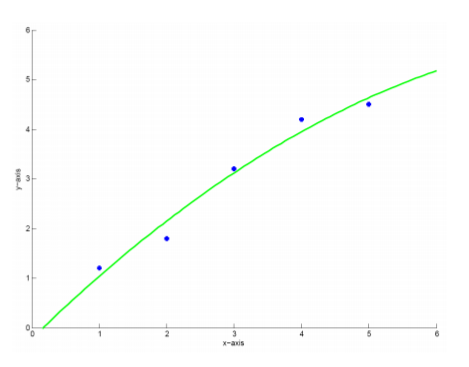
\includegraphics[height=5cm,keepaspectratio]{poly}

데이터 $(x_i, y_i), i=1,2,...,n$이 주어졌을 때, 이 데이터를 가장 잘 설명하는 p차함수 $y(x) = a_ix^i$를 찾아보자. 
\end{frame}


\begin{frame}{Motivation : Polynomial Regression} 
위와 비슷하게, 다음 LLS 문제로 볼 수 있다. 
\vspace{5mm}

$ \left| \left[ \begin{matrix} 
x_1^p & x_1^{p-1} & ... & x_1 & 1 \\  
x_2^p & x_2^{p-1} & ... & x_2 & 1 \\
... & ... & ... & ... & ... \\
x_n^p & x_n^{p-1} & ... & x_n & 1 
\end{matrix} \right] \left[ \begin{matrix} 
a_p \\
a_{p-1} \\
... \\ 
a_1 \\
a_0 \end{matrix} \right] - \left[ \begin{matrix}
y_1 \\
y_2 \\ 
... \\ 
y_n \end{matrix} \right] \right|^2 
$ 을 최소로 만드는 $a_i$는?

\end{frame}

\begin{frame}{Motivation : Curve Regression} 
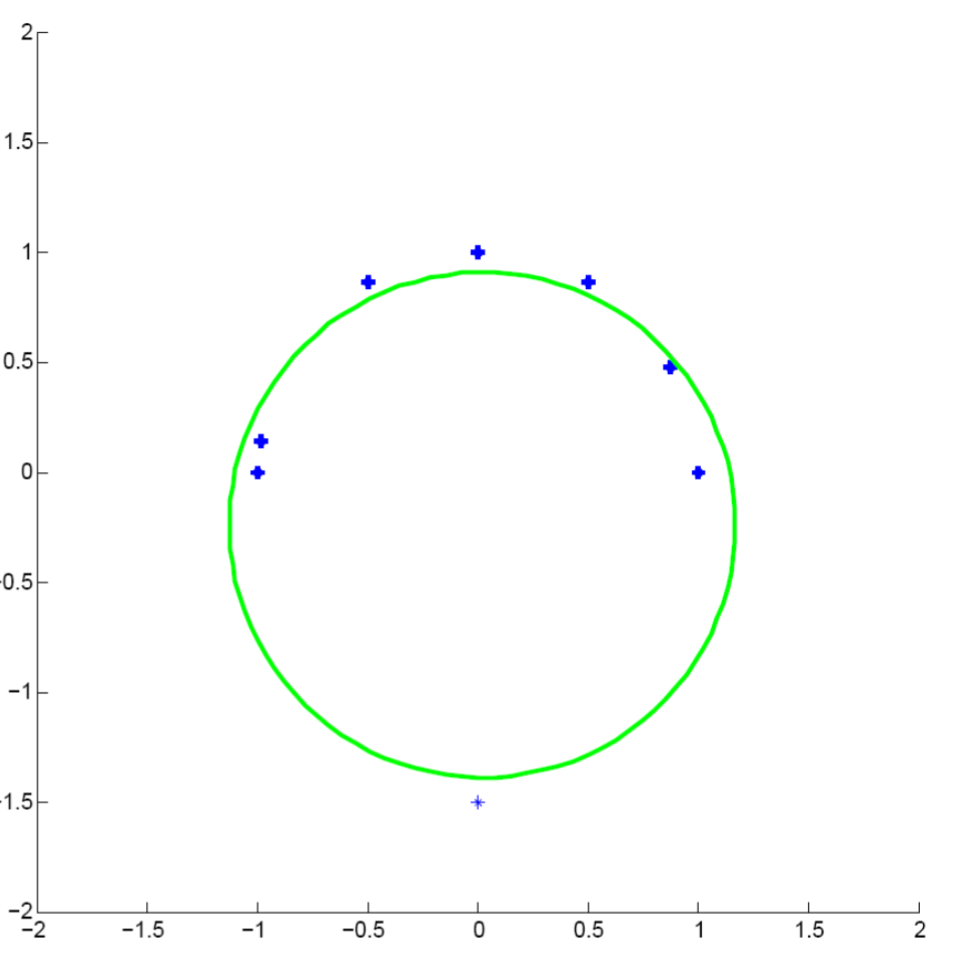
\includegraphics[height=5cm,keepaspectratio]{circle}

데이터 $(x_i, y_i), i=1,2,...,n$이 주어졌을 때, 가장 적절한 $(x-c_1)^2 + (y-c_2)^2 = r^2$을 찾아라. 
\end{frame}


\begin{frame}{Motivation : Polynomial Regression} 
이 문제 역시 LLS 문제로 볼 수 있다. 위에서 원의 방정식을 전개하여 정리하면 $2xc_1 + 2yc_2 + (r^2-c_1^2-c_2^2) - (x^2 + y^2) = 0$  이므로, $c_3 = r^2 -c_1^2-c_2^2$이라고 하면 다음과 같은 LLS 문제가 된다. 
\vspace{5mm}

$ \left| \left[ \begin{matrix} 
2x_1 & 2y_1 &  1 \\  
2x_2 & 2y_2 &  1 \\  
... & ... & ... \\
2x_n & 2y_n &  1 
\end{matrix} \right] \left[ \begin{matrix} 
c_1 \\
c_2 \\
c_3 \end{matrix} \right] - \left[ \begin{matrix}
x_1^2 + y_1^2 \\
x_2^2 + y_2^2 \\
...\\
x_n^2 + y_n^2 \end{matrix} \right] \right|^2 
$ 을 최소로 만드는 $c_i$는?

\end{frame}

\begin{frame}[allowframebreaks]{Solving LLS : Theory} 
어떤 $\vec{x*}$이 LLS 문제 $ min_{\vec{x}} |A\vec{x} - \vec{b}|^2 $ 의 해라고 하자. 그렇다면 다음이 성립한다. 

\begin{equation} 
|A\vec{x*} - \vec{b}|^2  = min_{\vec{x}} |A\vec{x} - \vec{b}|^2 
\end{equation}

그렇다면, 임의의 $\vec{y} \in \mathds{R}^n$에 대해서, 

\begin{equation}
|A\vec{x*} - \vec{b}|^2  \leq |A(\vec{x*} + \vec{y}) - \vec{b}|^2 
\end{equation}
인데, 이 식의 좌변을 $|\vec{x}|^2 = \vec{x} \bullet \vec{x}$임을 이용하여 전개하면 다음과 같다. 

\begin{eqnarray*} 
&&|A(\vec{x*} + \vec{y}) - \vec{b}|^2  \\
&=& (A(\vec{x*} + \vec{y}) - \vec{b})^T (A(\vec{x*} + \vec{y}) - \vec{b}) \\ 
&=& ((\vec{x*} + \vec{y})^T A^T - \vec{b}^T) (A(\vec{x*} + \vec{y}) - \vec{b}) \\ 
&=& (\vec{x*} + \vec{y})^T A^T A(\vec{x*} + \vec{y}) - \vec{b}^T A(\vec{x*} + \vec{y}) -  (\vec{x*} + \vec{y})^T A^T \vec{b} + \vec{b}^T \vec{b} \\
&=& \vec{x*}^T A^T A\vec{x*} - 2\vec{x*}^T A^T \vec{b} + \vec{b}^T \vec{b} + 2\vec{y}^T A^T A\vec{x*} - 2\vec{y}^T A^T \vec{b} + \vec{y}^T A^T \vec{y} \\ 
&=& |A\vec{x*}-\vec{b}|^2 + 2\vec{y}^T (A^T A\vec{x*} -A^T\vec{b}) + |A\vec{y}|^2
\end{eqnarray*}
이다. 따라서 1) $0 \leq 2\vec{y}^T (A^T A\vec{x*} -A^T\vec{b}) + |A\vec{y}|^2$ 이여야 한다. 

이 때, $|A\vec{y}|^2$은 0 이상이므로 첫 번째 항 $2\vec{y}^T (A^T A\vec{x*} -A^T\vec{b})$을 보자. 만약 이 항이 충분히 큰 음수라면, 1)은 성립하지 않는다. 여기서,  $\vec{y}$가 사실 다음의 조건 2)를 만족하는 벡터였다고 생각하자. 

\begin{equation} 
\vec{y} = - \alpha (A^T A \vec{x*} - A^T \vec{b})
\end{equation} 

만약 그렇더라도, 임의의 벡터 $\vec{y}$에 대해서 1)이 다 성립해야 하므로 2)를 1)에 대입하여도 성립하여야 한다. 대임하여 계산하면 다음과 같은 결과가 나온다. 

\begin{eqnarray} 
&&2\vec{y}^T (A^T A\vec{x*} -A^T\vec{b}) + |A\vec{y}|^2 \\
&=& -2 \alpha |A^T A\vec{x*} - A^T \vec{b}|^2 + \alpha^2 |A(A^T A \vec{x*} - A^T \vec{b}|^2  
\end{eqnarray}

이 된다. 이 식은 $\alpha$에 대한 이차함수로 볼 수 있다. 이 때, 이 식이 항상 0 이상이 될 조건은 $a>0$일 때 $ax^2 - bx$가 0 이상일 조건과 같다. 즉, 판별식 $D = b^2-4ac = b^2$ 이 0 이하여야 한다. 따라서 b는 0이여야만 하는데, 원 식에서 b는 $|A^T A\vec{x*} - A^T \vec{b}|$ 이므로, LLS를 만족시키는 해 $\vec{x*}$는 

\begin{equation} 
A^T A\vec{x*} - A^T \vec{b} = \vec{0}
\end{equation}

이여야 한다. 

역으로, 어떤 벡터 $\vec{x*}$이 $A^T A\vec{x*} - A^T \vec{b} = \vec{0}$을 만족한다면, 임의의 벡터 $\vec{x}$ 에 대해서 $\vec{y} = \vec{x} - \vec{x*}$이라 하면 다음이 성립한다. 

\begin{eqnarray} 
|A\vec{x} - \vec{b}|^2 &=& |A\vec{x*} + A\vec{y} - \vec{b}|^2 \\ 
&=& |A\vec{x*}-b|^2 + 2\vec{y}^T(A^T A\vec{x*} - A^T\vec{b}) + |A\vec{y}|^2 \\ 
&=& |A\vec{x*}-b|^2 + |A\vec{y}|^2  \\
&\geq& |A\vec{x*}-b|^2 
\end{eqnarray}

따라서, $\vec{x*}$는 LLS의 해이다. 
\end{frame}

\begin{frame}{Solution of LLS}

위 슬라이드에서 볼 수 있듯이, LLS의 해는 $A^TA\vec{x} -  A^T\vec{b} = 0$을 만족하는 $\vec{x}$이다. 이제 이를 구하는 방법을 생각해 보자. 크게 두 가지 방법을 생각해볼 수 있다. 

\begin{itemize} 
\item 선형방정식 풀이를 이용\footnote{위 식에서 $A^TA$를 행렬 A의 Psuedoinverse라 한다.}
\item QR Decomposition의 적용 
\end{itemize}

선형방정식의 풀이는 이미 해보았으므로, QR Decomposition을 적용해 보겠다. 

\end{frame}


\begin{frame}[allowframebreaks]{Solving LLS with QR decomposition} 

먼저, $A = Q\left[ \begin{matrix} R\\ 0 \end{matrix} \right]$으로 분해하자. 이 때 Q는 orthogonal matrix이므로 다음이 성립한다. 

\begin{itemize}
\item $Q^T A = \left[ \begin{matrix} R\\ 0 \end{matrix} \right]$ 
\item $|(A\vec(x) - \vec{b})|^2 = |Q^T (A\vec(x) - \vec{b})|^2 $
\end{itemize}

가 성립한다. 

여기서 두 번째 식에 초점을 맞추어 보면, 다음과 같은 계산이 가능하다. 

\begin{eqnarray} 
|(A\vec(x) - \vec{b})|^2 &=& |Q^T(A\vec(x) - \vec{b})|^2 \\
&=& |Q^TA \vec(x) - \vec{b})|^2 \\
&=& \left|\left[ \begin{matrix} R\\ 0 \end{matrix} \right] \vec(x) - Q^T\vec{b})\right|^2 
\end{eqnarray}

여기서 $Q^T \vec{b} = \left[ \begin{matrix} c\\ d \end{matrix} \right]$ 로 분할하면 위 식은 다음과 같이 바뀐다. 

\begin{eqnarray} 
|A\vec{x} - \vec{b}|^2 &=& \left|\left[ \begin{matrix} R\\ 0 \end{matrix} \right] \vec{x} - \left[ \begin{matrix} c\\ d \end{matrix} \right])\right|^2 \\ 
&=& \left|\left[ \begin{matrix} R\vec{x}-c\\ -d \end{matrix} \right]\right|^2 \\ 
&=& |R\vec{x}-c|^2 + |d|^2 
\end{eqnarray}

이므로, $|R\vec{x}-c|^2 = 0$일 때 $|A\vec{x}-\vec{b}|^2$이 최소가 된다. 따라서 $\vec{x} = R^{-1}c$가 된다. 따라서 

\begin{equation} 
\vec{x} = R^{-1}c 
\end{equation}

이다. 

\end{frame}

\begin{frame}{Back to the Motivation : Linear Regression} 

Coding!

\end{frame}





% \begin{frame}{Image Compression Using SVD} 
% % https://docs.google.com/viewer?a=v&pid=sites&srcid=ZGVmYXVsdGRvbWFpbnxuYXNsdW5kZXJpY3xneDpkMTI4OTI1NTc4YjRlOGE

% \end{frame}





% \section{Generalized Vector}


% \begin{frame}{Generalized Arithematic Operations} 

% 이때까지 벡터, 행렬 등의 \textit{선형대수학적} 객체들의 더하기와 상수배의 operation에 대해서 다루었다. 이제 이 연산을 확장해 보자. 즉, 이제부터는 더하기, 곱하기 등은 굳이 사칙연산일 필요가 없다. 예컨대, 함수끼리의 곱셈을 다음과 같이 정의할 수도 있다. 

% $\int f \bullet g dx $ 

% 더하기 역시 정의하기 나름이다. 이제부터 이러한 일반화된 사칙연산을 고려하기 위한 체계를 세워보겠다. 

% \end{frame}

% % \begin{frame}{Field} 

% % Field는 집합 하나와 그 집합의 원소간의 6개의 연산으로 정의된다. 

% % \begin{itemize} 
% % \item binary 연산 2개 : 더하기/곱하기 
% % \item unary 연산 2개 : 덧셈의 역원/곱셈의 역원 
% % \item constant 연산 2개 : 덧셈의 항등원(0) / 곱셈의 항등원(1)
% % \end{itemize}

% % 이 때, binary 연산은 교환법칙과 결합법칙이 성립해야 하며, 연산의 결과는 언제나 집합의 원소여야만 한다. 

% % \end{frame}

% \begin{frame}{항등원과 역원} 
% 어떤 집합 S에서의 이항연산 f에 대해서, 

% \begin{itemize} 
% \item 집합 S의 모든 원소 s에 대해서 f(s,i) = f(i,s) = s 이면 i를 그 연산의 항등원이라고 한다. 
% \item 집합 S의 어떤 원소 s에 대해서 f(s, t) = f(t, s) = i 이면 t를 s의 역원이라고 한다. 
% \end{itemize}
% \end{frame}

% \begin{frame}{Generalized Vector Space} 

% 어떤 집합 F 위에서 정의된 벡터공간 V는 어떤 집합 V와 F의 원소 a,b 와 V의 원소 $\vec{v}, \vec{u}$에 대해서 다음이 성립하는 벡터연산 더하기와 스칼라곱, 그리고 덧셈의 역원으로 정의된다. 이 때, F를 이 벡터공간의 스칼라라고 한다. 

% \begin{itemize} 
% \item 벡터덧셈의 교환법칙 / 결합법칙 
% \item 벡터덧셈의 항등원 / 역원
% \item 스칼라의 곱셈에서의 항등원 1에 대해서, $1\vec{v} = \vec{v}$
% \item $(ab)\vec{v} = a(b\vec{v})$ 
% \item $a(\vec{v} + \vec{u}) = a\vec{v} + a\vec{u} $
% \item $(a+b)\vec{v} = a\vec{v} + b\vec{v}$
% \end{itemize}

% 여기서, 스칼라곱과 벡터-스칼라곱이나 스칼라끼리의 합과 벡터-벡터간의 합은 다른 operation이다. 

% \end{frame}

% % https://math.okstate.edu/people/binegar/3013-S99/3013-l12.pdf
% \begin{frame}{Examples of an Abstract Vector Space} 
% \begin{itemize} 
% \item Polynomials with degree $\leq n$
% \item Matrices
% \item Linear Transformations
% \item Functions from a specific domain (will be revisited after few weeks)
% \item Random Variables (will be revisited after few weeks)
% \end{itemize}
% \end{frame}

% \begin{frame}{예시 : $\mathds{R}^2$에서 $\mathds{R}^2$로의 선형변환}

% $\mathds{R}^2$에서 $\mathds{R}^2$로의 선형변환은 2 by 2 행렬로 나타내어질 수 있다. 따라서, 행렬의 덧셈과 실수배를 이용하여 선형변환의 벡터공간을 정의할 수 있다. 이제부터 이 공간의 기저와 좌표, 그리고 2차원 좌표계에서 선형변환 벡터들이 어떠한 의미를 가지는지를 알아볼 것이다. 

% \end{frame}

% \begin{frame}{예시 : $\mathds{R}^2$에서 $\mathds{R}^2$로의 선형변환} 
% 먼저, 다음의 행렬들을 생각해 보자. 
% $ \vec{e}_1 =  
% \left[ \begin{matrix}
% 1 & 0  \\
% 0 & 0 
% \end{matrix} \right],
% \vec{e}_2 = 
% \left[ \begin{matrix}
% 0 & 1  \\
% 0 & 0 
% \end{matrix} \right],
% \vec{e}_3 = 
% \left[ \begin{matrix}
% 0 & 0  \\
% 1 & 0 
% \end{matrix} \right],
% \vec{e}_3 = 
% \left[ \begin{matrix}
% 0 & 0  \\
% 0 & 1 
% \end{matrix} \right]
% $

% 이 행렬들은 명백하게 2 by 2 행렬이므로, $\mathds{R}^2$에서 $\mathds{R}^2$로의 선형변환이다. 이들 벡터는 선형독립일까? 또, 위 4개의 벡터는 기저가 될까? 
% \end{frame}

% \begin{frame}{Linear Independence of an Abstract Vector Space}
% 위 4개의 벡터가 선형독립이기 위해서는 $c_ie_i$을 만족하는 $c_i$가 0뿐이여야 한다. 위 경우, 

% $c_i\vec{e}_i = \left[ \begin{matrix}
% c_1 & c_2  \\
% c_3 & c_4 
% \end{matrix} \right]$ 이므로 선형독립임을 알 수 있다. 

% 또한, 임의의 2 by 2 행렬을 $c_i$를 적절히 조정하여 만들 수 있으므로, 기저임을 알 수 있다. 
% \end{frame}



% \begin{frame}{예시 : $\mathds{R}^2$에서 $\mathds{R}^2$로의 선형변환} 

% 위와 같이 선형변환의 기저를 찾은 것은 어떤 의미가 있을까? 

% 이는 이제부터 우리가 $\mathds{R}^2$의 한 점에서 $\mathds{R}^2$의 한 점으로 대응시키는 선형변환을 언제나 4개의 선형변환을 조합하여 하는 것으로 이해할 수 있다는 점이다. 
% \end{frame}


% \begin{frame}{Extending an Abstract Vector Space : Inner Product Space} 
% 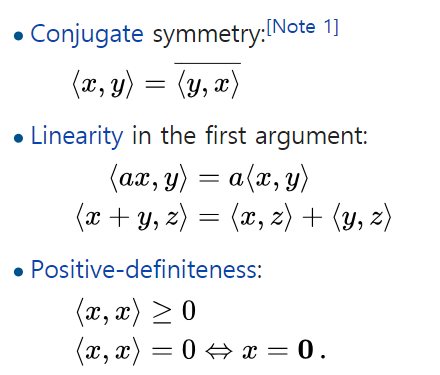
\includegraphics[width=10cm,keepaspectratio]{innerproduct}
% \end{frame}

% \begin{frame}{Abstract Vector Space vs $\mathds{R}^n$}

% \end{frame}


% \begin{frame}{Isomorphism Between Vector Spaces}
% \end{frame}


% \section{극한}

% \begin{frame}{극한의 정의}

% \end{frame}

% \begin{frame}{식의 극한}

% \end{frame}

\end{document}


